Problemem w poprawnym opisie zależności między zmiennymi losowymi jest fakt, że dostępnych mamy wiele statystyk które ją mierzą. Każda z nich uchwyca pewien konkretny aspekt współzależności, i nie da się jasno wyróżnić konkretnej jako "najlepszej". W tej sekcji pracy zaprezentujemy wybrane narzędzia służące do badania struktury zależności zmiennych losowych.

\subsubsection{$\rho$ Pearsona}
Podstawową i najbardziej znaną miarą współzależności zmiennych losowych jest korelacja Pearsona.

\begin{df}[Korelacja Pearsona]
	Niech $X$ i $Y$ będą zmiennymi losowymi o skończonych drugich momentach. Współczynnikiem korelacji pearsona $\rho$ nazywamy
	
	$$ \rho(X, Y) \coloneqq \Corr(X,Y) = \frac{\Cov(X,Y)}{\sqrt{\Var(X)}\sqrt{\Var(Y)}}.$$
\end{df}

Ten współczynnik korelacji przyjmuje wartości z zakresu $[-1, 1]$, gdzie $\vert\rho\vert=1$ oznacza idealną liniową relację. Korelacja pearsona jest podstawową miarą zależności podawaną w każdym podręczniku do statystyki. Ma jednak szereg wad: nie jest zdefiniowana dla ciężkoogonowych rozkładów (przez nieokreśloną wariancję), oraz jest wrażliwa na monotonicznie rosnące przekształcenia $X$ i $Y$. Te i wiele innych ograniczeń korelacji pearsona stoi w sprzeczności z aksjomatycznym podejściem do miar zgodności (czyt. \ref{def:miara_zgodnosci}). \\
Gdy w rozdziale \ref{subsec:dwuwymiarowe_kopuly_definicja} zdefiniujemy czym jest główny obiekt tej pracy, czyli kopuła, zależeć nam będzie, żeby móc opisać zależność zmiennych losowych $X$, $Y$ w terminach łączącej je kopuły $C$. Z tego powodu, interesujące dla nas będą miary zależności, które są niezmiennicze na monotonicznie rosnące przekształcenia (ze względu na transformację PIT \ref{def:PIT}, czyt. rozdział \ref{subsec:dwuwymiarowe_kopuly_definicja}). Korelacja pearsona nam tego nie zapewni, ale możemy zdefiniować inne miary: zgodności zmiennych losowych, które posiadają lepsze własności z punktu widzenia teorii kopuł.\\

Aby w pełni zdefiniować aksjomatyczne podejście do miar zgodności jak wprowadził to Scarsini w \cite{Scarsini1984}, potrzebujemy mieć dostępne pojęcie kopuły. W tej pracy formalnie zostaną one wprowadzone dopiero w definicji \ref{def:bivariate_copula}, w związku z czym na ten moment powiemy jedynie (nieformalnie), że kopuła jest funkcją która opisuje charakter i siłę zależności między zmiennymi losowymi. Pełną definicję i opis czym są kopuły można przeczytać w rozdziale \ref{sec:dwuwymiarowe_kopuly}.

\begin{df}[Miara zgodności]
	Rozpatrzmy zmienne losowe $X$ i $Y$ powiązane kopułą $C$. $M_{X,Y}=M_C$ nazwiemy miarą zgodności, wtedy i tylko wtedy gdy:
	\begin{enumerate}
		\item jest zdefiniowana dla dowolnych zmiennych $X$, $Y$
		\item jest relatywna, lub znormalizowana: $M_{X,Y}\in[-1,1]$
		\item jest symetryczna: $M_{X,Y}=M_{Y,X}$
		\item jeśli $X$ i $Y$ są niezależne, to $M_{X,Y}=0$
		\item $M_{-X,Y}=M_{X,-Y}=-M_{Y,X}$
		\item jest zbieżna, gdy kopuła jest punktowo zbieżna, tzn. jeśli $\{(X_n,Y_n)\}$ jest ciągiem ciągłych zmiennych losowych o kopułach $\{C_n\}$, oraz 
		$$ \lim\limits_{n\to\infty} C_n(u, v) =C(u, v)\text{, dla każdych }(u, v)\in[0,1]^2,$$
		to wtedy
		$$ \lim\limits_{n\to\infty}M_{X_n,Y_n}=M_{X,Y}.$$
		\item przestrzega relacji zgodności: jeśli $C_1(u,v) \leqslant C_2(u,v)$ dla wszystkich $(u, v)\in[0,1]^2$, to $M_{C_1} \leqslant M_{C_2}.$
	\end{enumerate}
	\label{def:miara_zgodnosci}		
\end{df}

Aksjomatyczne podejście z powyższej definicji zawęża przestrzeń miar zgodności do takich, które są niezmiennicze względem rosnących transformacji, czyli:
$$ M_{X,Y} = M_{\alpha(X), \beta(Y)},$$
dla dowolnych funkcji $\alpha,\beta$ rosnących prawie wszędzie.\\

\subsubsection{Współmonotoniczność i przeciwmonotoniczność}
Współmonotoniczność i przeciwmonotoniczność to szczególne przypadki zależności zmiennych losowych, w których są one od siebie perfekcyjnie zależne.

\begin{df}[Zbiór współmonotoniczny]
	Zbiór $A \subset \R^2$ nazywamy współmonotonicznym, wtedy i tylko wtedy gdy dla dowolnych $(x_1, y_1)$, $(x_2, y_2)$ z $A$ zachodzi:
	
	$$ (x_1 - y_1)(x_2 - y_2) >0.$$
\end{df}

\begin{df}[Zbiór przeciwmonotoniczny]
	Zbiór $A \subset \R^2$ nazywamy przeciwmonotonicznym, wtedy i tylko wtedy gdy dla dowolnych $(x_1, y_1)$, $(x_2, y_2)$ z $A$ zachodzi:
	
	$$ (x_1 - y_1)(x_2 - y_2) <0.$$
\end{df}


\begin{df}[Zmienne losowe współ- i przeciwmonotoniczne]
	Wektor losowy $(X, Y)$ nazywamy współmonotonicznym (przeciwmonotonicznym), lub perfekcyjnie dodatnio (ujemnie) zależnym wtedy i tylko wtedy gdy istnieje zbiór współmonotoniczny (przeciwmonotoniczny) $A\subset\R^2$:
	
	$$ \Pra[(X,Y)\in A]=1.$$
\end{df}

Współmonotoniczność i przeciwmonotoniczność zmiennych losowych jest ważnym konceptem w teorii kopuł, ponieważ definiuje najsilniejszy rodzaj zależności jakie kopuły mogą reprezentować (czyt. twierdzenie \ref{thm:frechet_hoeffding}).

\subsubsection{$\tau$ Kendalla i $\rho$ Spearmana}

Współczynniki $\tau$ Kendalla i $\rho$ Spearmana oba spełniają aksjomaty miar zgodności z \cite{Scarsini1984}. Są współczynnikami rangowymi, więc nie zależą od monotonicznych przekształceń rozkładów brzegowych $X$ czy $Y$. Ich zaletą jest to, że mogą być przez to jednoznacznie przedstawione w języku kopuły - co znajduje zastosowanie przy estymacji parametrów modeli kopułowych. Ta własność zazwyczaj nie zachodzi w przypadku korelacji Pearsona.

\begin{df}[$\tau$ Kendalla]
	Współczynnik $\tau$ Kendalla między ciągłymi zmiennymi losowymi $X$ i $Y$ o kopule definiujemy jako:
	$$ \tau = \Pra[(X_1-X_2)(Y_1-Y_2)>0] - \Pra[(X_1-X_2)(Y_1-Y_2) <0], $$
	gdzie $(X_1, Y_1)$ i $(X_2, Y_2)$ są kopiami iid wektora $(X, Y)$.
\end{df}

\begin{df}[$\rho$ Spearmana]
	Współczynnik $\rho$ Spearmana między ciągłymi zmiennymi losowymi $X$ i $Y$ o rozkładach brzegowych $F_X$ i $F_y$ zadany jest przez:
	$$ \rho = \Corr[F_X(X), F_Y(Y)].$$
\end{df}

Współczynniki te dają się jednoznacznie wyrazić za pomocą kopuł łączących $X$~i~$Y$~-~własność tę podamy w rozdziale \ref{subsec:dwuwymiarowe_kopuly_definicja}. Istotny również jest fakt, że ich ekstremalne wartości, tj. $\rho= 1$, czy $\tau=1$ odpowiadają współmonotoniczności zmiennych losowych, a $\rho=-1$, czy $\tau=-1$ odpowiadają przeciwmonotoniczności.

\subsubsection{Zależność ogonów}
Na zależność zmiennych losowych można popatrzeć również ze strony zależności obserwacji ekstremalnych. Rozważmy następującą statystykę:

\begin{df}[Współczynnik zależności ogonów]
	Górnym współczynnikiem zależności ogonów $(X_1, X_2)$ o rozkładach brzegowych $F_1$ i $F_2$ i kopuli $C$ nazywamy:
	$$ \lambda^{u} = \lim\limits_{t\to1^{-}}\Pra[X_2 > F_2^{-1}(t) \vert X_1 > F_1^{-1}(t) ].$$
	Dolnym współczynnikiem nazywamy:
	$$ \lambda^{l} = \lim\limits_{t\to0^{+}}\Pra[X_2 \leqslant F_2^{-1}(t) \vert X_1 \leqslant F_1^{-1}(t) ].$$
\end{df}

Współczynniki zależności ogonów informują o sile zależności zmiennych losowych w granicy, gdy dążymy z jedną z nich coraz dalej w jej ogon. Mówimy, że zmienne losowe posiadają zależność ogonów jeśli $\lambda \in (0, 1]$, lub jej nie posiadają gdy $\lambda =0$. Te wspołczynniki zależą przede wszystkim od obserwacji będących ekstremalnymi względem obu zmiennych. Rysunek \ref{fig:tail_dependence} prezentuje przykładowy rozkład posiadający dolny współczynnik zależności ogonów, lecz nie posiadający górnego wspołczynnika. Kolorami zaznaczone są obserwacje które wpływają na dolny (szare punkty) i górny (czerwone punkty) współczynnik zależności ogonów.\\
W praktycznych zastosowaniach, jest on jednak trudny do kalibracji z danych - koncept ten działa raczej w drugą stronę: z parametrów skalibrowanego modelu implikowany jest współczynnik zależności ogonów.
\begin{figure}[H]
	\centering
	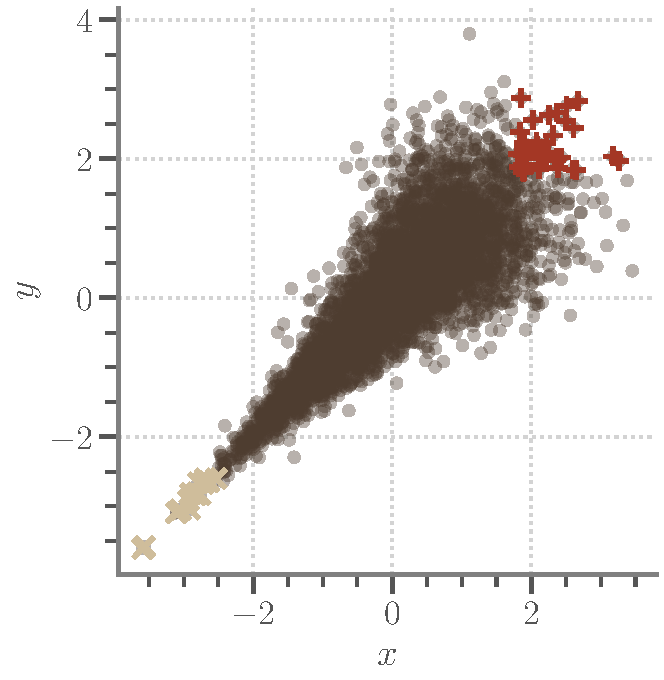
\includegraphics[width=0.5\linewidth]{01_Tail_dependence}	
	\caption{Ilustracja górnego i dolnego współczynnika zależności ogonów.\label{fig:tail_dependence}}
\end{figure}

W tym rozdziale zdefiniowialiśmy różne miary pomagające nam zrozumieć zależność zmiennych losowych. Widzimy zatem, że korelacja Pearsona i modele eliptyczne to za mało, aby w pełni uchwycić charakter współzależności. W kolejnym rozdziale podamy teorię \emph{kopuł}, które dadzą nam odpowiednie narzędzia do walki z tym problemem.